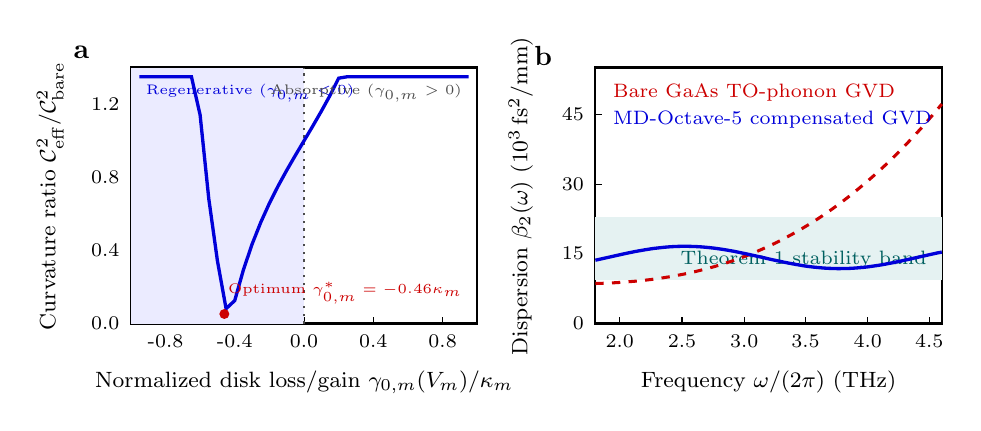
\begin{tikzpicture}[x=1cm,y=1cm,font=\footnotesize]
  % Panel a: Curvature cancellation vs normalized micro-disk bias gamma_0 / kappa
  \node[anchor=north west,font=\bfseries\normalsize] at (0.10,4.35) {a};
  \draw[thick] (0.95,0.70) rectangle (5.35,3.95);
  \foreach \v/\y in {0.0/0.70, 0.4/1.63, 0.8/2.56, 1.2/3.49} {
    \draw (0.95,\y) -- (1.03,\y);
    \node[left,font=\scriptsize] at (0.93,\y) {\v};
  }
  \foreach \xval/\xpos in {-0.8/1.39, -0.4/2.27, 0.0/3.15, 0.4/4.03, 0.8/4.91} {
    \draw (\xpos,0.70) -- (\xpos,0.78);
    \node[below,font=\scriptsize] at (\xpos,0.68) {\xval};
  }
  \node[below,font=\footnotesize] at (3.15,0.22) {Normalized disk loss/gain $\gamma_{0,m}(V_m)/\kappa_m$};
  \node[rotate=90,above,font=\footnotesize] at (0.22,2.32) {Curvature ratio $\mathcal{C}_{\mathrm{eff}}^2/\mathcal{C}_{\mathrm{bare}}^2$};

  % Shaded regenerative amplification window (-1 < gamma_0/kappa < 0)
  \fill[blue!8] (0.95,0.70) rectangle (3.15,3.95);
  \draw[dotted,black!70,line width=0.8pt] (3.15,0.70) -- (3.15,3.95);
  \draw[blue!85!black,line width=1.2pt] (1.060,3.834) -- (1.170,3.834) -- (1.280,3.834) -- (1.390,3.834) -- (1.500,3.834) -- (1.610,3.834) -- (1.720,3.834) -- (1.830,3.349) -- (1.940,2.286) -- (2.050,1.496) -- (2.160,0.888) -- (2.270,0.992) -- (2.380,1.382) -- (2.490,1.707) -- (2.600,1.984) -- (2.710,2.227) -- (2.820,2.445) -- (2.930,2.646) -- (3.040,2.836) -- (3.150,3.021) -- (3.260,3.206) -- (3.370,3.397) -- (3.480,3.597) -- (3.590,3.816) -- (3.700,3.834) -- (3.810,3.834) -- (3.920,3.834) -- (4.030,3.834) -- (4.140,3.834) -- (4.250,3.834) -- (4.360,3.834) -- (4.470,3.834) -- (4.580,3.834) -- (4.690,3.834) -- (4.800,3.834) -- (4.910,3.834) -- (5.020,3.834) -- (5.130,3.834) -- (5.240,3.834);
  \fill[red!80!black] (2.138,0.821) circle (1.8pt);

  \node[anchor=north west,font=\tiny,blue!85!black] at (1.02,3.86) {Regenerative ($\gamma_{0,m}<0$)};
  \node[anchor=south east,font=\tiny,red!80!black] at (5.28,0.82) {Optimum $\gamma_{0,m}^*=-0.46\kappa_m$};
  \node[anchor=north east,font=\tiny,black!70] at (5.28,3.86) {Absorptive ($\gamma_{0,m}>0$)};

  % Panel b: Group-velocity dispersion beta_2(omega) across 1.9-4.5 THz
  \node[anchor=north west,font=\bfseries\normalsize] at (5.95,4.35) {b};
  \draw[thick] (6.85,0.70) rectangle (11.25,3.95);
  \foreach \v/\y in {0/0.70, 15/1.59, 30/2.47, 45/3.36} {
    \draw (6.85,\y) -- (6.93,\y);
    \node[left,font=\scriptsize] at (6.83,\y) {\v};
  }
  \foreach \fval/\xpos in {2.0/7.16, 2.5/7.95, 3.0/8.74, 3.5/9.52, 4.0/10.31, 4.5/11.09} {
    \draw (\xpos,0.70) -- (\xpos,0.78);
    \node[below,font=\scriptsize] at (\xpos,0.68) {\fval};
  }
  \node[below,font=\footnotesize] at (9.05,0.22) {Frequency $\omega/(2\pi)$ (THz)};
  \node[rotate=90,above,font=\footnotesize] at (6.18,2.32) {Dispersion $\beta_2(\omega)$ ($10^3\,\mathrm{fs^2/mm}$)};

  \fill[teal!10] (6.85,1.25) rectangle (11.25,2.05);
  \node[anchor=south east,font=\scriptsize,teal!75!black] at (11.18,1.28) {Theorem 1 stability band};

  \draw[red!80!black,dashed,line width=1.1pt] (6.850,1.208) -- (6.913,1.210) -- (6.976,1.212) -- (7.039,1.215) -- (7.101,1.218) -- (7.164,1.222) -- (7.227,1.227) -- (7.290,1.232) -- (7.353,1.237) -- (7.416,1.243) -- (7.479,1.250) -- (7.541,1.257) -- (7.604,1.265) -- (7.667,1.274) -- (7.730,1.284) -- (7.793,1.294) -- (7.856,1.305) -- (7.919,1.317) -- (7.981,1.329) -- (8.044,1.343) -- (8.107,1.357) -- (8.170,1.372) -- (8.233,1.388) -- (8.296,1.405) -- (8.359,1.422) -- (8.421,1.441) -- (8.484,1.460) -- (8.547,1.481) -- (8.610,1.502) -- (8.673,1.525) -- (8.736,1.548) -- (8.799,1.573) -- (8.861,1.598) -- (8.924,1.625) -- (8.987,1.653) -- (9.050,1.681) -- (9.113,1.711) -- (9.176,1.742) -- (9.239,1.775) -- (9.301,1.808) -- (9.364,1.842) -- (9.427,1.878) -- (9.490,1.915) -- (9.553,1.953) -- (9.616,1.992) -- (9.679,2.032) -- (9.741,2.074) -- (9.804,2.117) -- (9.867,2.161) -- (9.930,2.207) -- (9.993,2.254) -- (10.056,2.302) -- (10.119,2.352) -- (10.181,2.403) -- (10.244,2.455) -- (10.307,2.509) -- (10.370,2.564) -- (10.433,2.620) -- (10.496,2.678) -- (10.559,2.737) -- (10.621,2.798) -- (10.684,2.860) -- (10.747,2.924) -- (10.810,2.989) -- (10.873,3.056) -- (10.936,3.124) -- (10.999,3.193) -- (11.061,3.265) -- (11.124,3.337) -- (11.187,3.412) -- (11.250,3.487);
  \draw[blue!85!black,line width=1.2pt] (6.850,1.504) -- (6.913,1.518) -- (6.976,1.532) -- (7.039,1.546) -- (7.101,1.560) -- (7.164,1.574) -- (7.227,1.588) -- (7.290,1.601) -- (7.353,1.614) -- (7.416,1.625) -- (7.479,1.636) -- (7.541,1.646) -- (7.604,1.655) -- (7.667,1.662) -- (7.730,1.669) -- (7.793,1.674) -- (7.856,1.678) -- (7.919,1.680) -- (7.981,1.681) -- (8.044,1.680) -- (8.107,1.678) -- (8.170,1.675) -- (8.233,1.670) -- (8.296,1.664) -- (8.359,1.657) -- (8.421,1.648) -- (8.484,1.639) -- (8.547,1.628) -- (8.610,1.617) -- (8.673,1.604) -- (8.736,1.591) -- (8.799,1.578) -- (8.861,1.564) -- (8.924,1.550) -- (8.987,1.536) -- (9.050,1.521) -- (9.113,1.507) -- (9.176,1.494) -- (9.239,1.480) -- (9.301,1.468) -- (9.364,1.456) -- (9.427,1.445) -- (9.490,1.434) -- (9.553,1.425) -- (9.616,1.417) -- (9.679,1.411) -- (9.741,1.405) -- (9.804,1.401) -- (9.867,1.399) -- (9.930,1.397) -- (9.993,1.398) -- (10.056,1.399) -- (10.119,1.402) -- (10.181,1.407) -- (10.244,1.412) -- (10.307,1.419) -- (10.370,1.428) -- (10.433,1.437) -- (10.496,1.447) -- (10.559,1.459) -- (10.621,1.471) -- (10.684,1.484) -- (10.747,1.497) -- (10.810,1.511) -- (10.873,1.525) -- (10.936,1.539) -- (10.999,1.553) -- (11.061,1.567) -- (11.124,1.581) -- (11.187,1.595) -- (11.250,1.607);

  \node[anchor=north west,font=\scriptsize,red!80!black] at (6.95,3.86) {Bare GaAs TO-phonon GVD};
  \node[anchor=north west,font=\scriptsize,blue!85!black] at (6.95,3.52) {MD-Octave-5 compensated GVD};
\end{tikzpicture}
